% questions.tex —— 2010 年·普通高等学校招生考试·四川卷·理科 · 题目内容片段（无答案）
% 由 tools/generate_projects.py 依来源总账自 2010/2010_数学真题_四川理_试题.md 生成，勿手改（改源 MD 后重跑）


状态：needs-review；依固定候选 PDF 两页（印刷页 631–632）逐题核验，四幅图已矢量重绘。原页未印分值，不补。

\gkpart{一、选择题}

\begin{question}
\gkti{1}$i$ 是虚数单位，计算 $i+i^2+i^3=$（　）

（A）$-1$

（B）$1$

（C）$-i$

（D）$i$

\Needspace{0.4\textheight}
\end{question}
\begingroup
\renewenvironment{question}{\Needspace{0.5\textheight}}{}
\begin{question}
\gkti{2}下列四个图象所表示的函数，在点 $x=0$ 处连续的是（　）
\nopagebreak[4]
\begin{center}% 2010 年四川卷理科第 2 题：四个函数图象选项（A）—（D）。
% 来源 PDF：普通高考/2010/2010四川理.pdf，SHA-256 499425696359cfc2cf4418254bdaa1a37487b3dbaa072ff3c7cbe18dbabe73dc。
% 原页：第 1 页（A3 三栏）第 1 栏中部，书页码 631。
% 重绘依据：原页为两行两列四幅图象，均只画坐标系与曲线、不标刻度；
%   (A) 双曲线型，x=0 左右两支各自趋于无穷，无定义点；
%   (B) 递增曲线在 x=0 处挖去一点（空心圈），极限存在但函数值缺失；
%   (C) y=|x| 形状，原点挖空、另在 y 轴负半轴实心一点；
%   (D) 左支曲线渐平后自 x=0 起接一条下降直线，两段在该点相接，连续。
\begin{tikzpicture}[semithick, every node/.style={inner sep=1.2pt, font=\small}]
  % ===== (A)：双曲线型，x=0 处两侧都趋于无穷
  \draw[-stealth] (0.25,1.40) -- (4.00,1.40);
  \draw[-stealth] (1.55,0.05) -- (1.55,3.15);
  \draw[thick,domain=1.67:3.85,samples=80] plot (\x,{1.40+0.25/(\x-1.55)});
  \draw[thick,domain=0.30:1.28,samples=80] plot (\x,{1.40-0.25/(1.55-\x)});
  \node[below left] at (1.55,1.40) {$O$};
  \node[left] at (1.55,3.15) {$y$};
  \node[below] at (4.00,1.40) {$x$};
  \node at (2.05,-0.45) {（A）};

  % ===== (B)：递增曲线，x=0 处为空心圈
  \draw[-stealth] (5.85,1.40) -- (9.60,1.40);
  \draw[-stealth] (7.15,0.05) -- (7.15,3.15);
  \draw[thick,domain=5.95:8.55,samples=100]
    plot (\x,{1.72+0.50*(\x-7.15)+0.18*(\x-7.15)*(\x-7.15)*(\x-7.15)});
  \draw[fill=white,thick] (7.15,1.72) circle (2.2pt);
  \node[below right] at (7.15,1.40) {$O$};
  \node[left] at (7.15,3.15) {$y$};
  \node[below] at (9.60,1.40) {$x$};
  \node at (7.65,-0.45) {（B）};

  % ===== (C)：y=|x| 形状，原点挖空、y 轴负半轴另有实心点
  \draw[-stealth] (0.25,-2.15) -- (4.00,-2.15);
  \draw[-stealth] (1.55,-3.45) -- (1.55,-0.95);
  \draw[thick] (0.35,-0.95) -- (1.55,-2.15);
  \draw[thick] (1.55,-2.15) -- (2.75,-0.95);
  \draw[fill=white,thick] (1.55,-2.15) circle (2.2pt);
  \fill (1.55,-2.75) circle (1.6pt);
  \node[below left] at (1.55,-2.15) {$O$};
  \node[left] at (1.55,-0.95) {$y$};
  \node[below] at (4.00,-2.15) {$x$};
  \node at (2.05,-3.95) {（C）};

  % ===== (D)：左支渐平、x=0 处接一条下降直线
  \draw[-stealth] (5.85,-2.15) -- (9.60,-2.15);
  \draw[-stealth] (7.15,-3.45) -- (7.15,-0.95);
  \draw[thick,domain=5.95:7.15,samples=80]
    plot (\x,{-2.02+0.95*((7.15-\x)/1.20)*((7.15-\x)/1.20)});
  \draw[thick] (7.15,-2.02) -- (8.45,-3.18);
  \node[below left] at (7.15,-2.15) {$O$};
  \node[left] at (7.15,-0.95) {$y$};
  \node[below] at (9.60,-2.15) {$x$};
  \node at (7.65,-3.95) {（D）};
\end{tikzpicture}
\end{center}
\nopagebreak[4]
\end{question}
\endgroup
\begin{question}
\gkti{3}$2\log_510+\log_50.25=$（　）

（A）$0$

（B）$1$

（C）$2$

（D）$4$

\end{question}
\begin{question}
\gkti{4}函数 $f(x)=x^2+mx+1$ 的图象关于直线 $x=1$ 对称的充要条件是（　）

（A）$m=-2$

（B）$m=2$

（C）$m=-1$

（D）$m=1$

\end{question}
\begin{question}
\gkti{5}设点 $M$ 是线段 $BC$ 的中点，点 $A$ 在直线 $BC$ 外，$\overrightarrow{BC}^2=16$，$\left|\overrightarrow{AB}+\overrightarrow{AC}\right|=\left|\overrightarrow{AB}-\overrightarrow{AC}\right|$，则 $\left|\overrightarrow{AM}\right|=$（　）

（A）$8$

（B）$4$

（C）$2$

（D）$1$

\end{question}
\begin{question}
\gkti{6}将函数 $y=\sin x$ 的图象上所有的点向右平行移动 $\dfrac{\pi}{10}$ 个单位长度，再把所得各点的横坐标伸长到原来的 $2$ 倍（纵坐标不变），所得图象的函数解析式是（　）

（A）$y=\sin\left(2x-\dfrac{\pi}{10}\right)$

（B）$y=\sin\left(2x-\dfrac{\pi}{5}\right)$

（C）$y=\sin\left(\dfrac{1}{2}x-\dfrac{\pi}{10}\right)$

（D）$y=\sin\left(\dfrac{1}{2}x-\dfrac{\pi}{20}\right)$

\end{question}
\begin{question}
\gkti{7}某加工厂用某原料由甲车间加工出 $A$ 产品，由乙车间加工出 $B$ 产品。甲车间加工一箱原料需耗费工时 $10$ 小时可加工出 $7$ 千克 $A$ 产品，每千克 $A$ 产品获利 $40$ 元。乙车间加工一箱原料需耗费工时 $6$ 小时可加工出 $4$ 千克 $B$ 产品，每千克 $B$ 产品获利 $50$ 元。甲、乙两车间每天共能完成至多 $70$ 箱原料的加工，每天甲、乙两车间耗费工时总和不得超过 $480$ 小时，甲、乙两车间每天总获利最大的生产计划为（　）

（A）甲车间加工原料 $10$ 箱，乙车间加工原料 $60$ 箱

（B）甲车间加工原料 $15$ 箱，乙车间加工原料 $55$ 箱

（C）甲车间加工原料 $18$ 箱，乙车间加工原料 $50$ 箱

（D）甲车间加工原料 $40$ 箱，乙车间加工原料 $30$ 箱

\end{question}
\begin{question}
\gkti{8}已知数列 $\{a_n\}$ 的首项 $a_1\neq0$，其前 $n$ 项和为 $S_n$，且 $S_{n+1}=2S_n+a_1$，则 $\lim\limits_{n\to\infty}\dfrac{a_n}{S_n}=$（　）

（A）$0$

（B）$\dfrac{1}{2}$

（C）$1$

（D）$2$

\end{question}
\begin{question}
\gkti{9}椭圆 $\dfrac{x^2}{a^2}+\dfrac{y^2}{b^2}=1$（$a>b>0$）的右焦点为 $F$，其右准线与 $x$ 轴的交点为 $A$，在椭圆上存在点 $P$ 满足线段 $AP$ 的垂直平分线过点 $F$，则椭圆离心率的取值范围是（　）

（A）$\left(0,\dfrac{\sqrt2}{2}\right]$

（B）$\left(0,\dfrac{1}{2}\right]$

（C）$[\sqrt2-1,1)$

（D）$\left[\dfrac{1}{2},1\right)$

\end{question}
\begin{question}
\gkti{10}由 $1,2,3,4,5,6$ 组成没有重复数字且 $1,3$ 都不与 $5$ 相邻的六位偶数的个数是（　）

（A）$72$

（B）$96$

（C）$108$

（D）$144$

\Needspace{0.4\textheight}
\end{question}
\begingroup
\renewenvironment{question}{\Needspace{0.5\textheight}}{}
\begin{question}
\gkti{11}半径为 $R$ 的球 $O$ 的直径 $AB$ 垂直于平面 $\alpha$，垂足为 $B$，$\triangle BCD$ 是平面 $\alpha$ 内边长为 $R$ 的正三角形，线段 $AC$、$AD$ 分别与球面交于点 $M$、$N$，那么 $M$、$N$ 两点间的球面距离是（　）
\nopagebreak[4]
\begin{center}% 2010 年四川卷理科第 11 题：球 O、直径 AB⊥平面 α 于 B，正三角形 BCD 在 α 内，
%   线段 AC、AD 与球面交于 M、N。
% 来源 PDF：普通高考/2010/2010四川理.pdf，SHA-256 499425696359cfc2cf4418254bdaa1a37487b3dbaa072ff3c7cbe18dbabe73dc。
% 原页：第 1 页（A3 三栏）第 2 栏中部，书页码 631。
% 重绘依据：球画成圆 + 赤道椭圆（后半虚线、前半实线）；平面 α 画成平行四边形，球与之相切于 B，
%   平面远边被球遮挡处留白；△BCD 整个落在平行四边形内（BC、CD 实线，BD 被球遮挡用虚线）；
%   AC、AD 在球内的部分（A—M、A—N）与直径 AB 同样画虚线，球外部分（M—C、N—D）画实线。
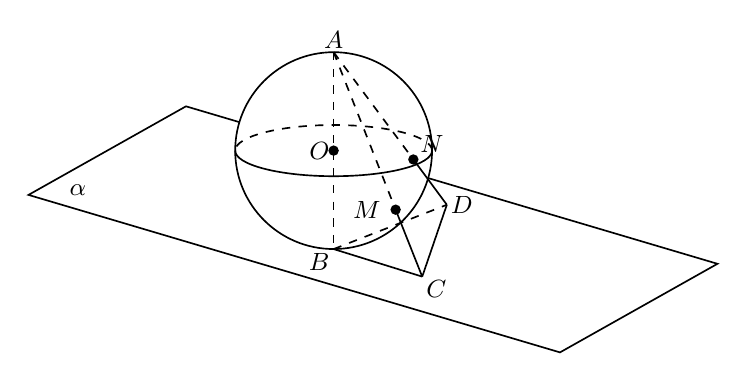
\begin{tikzpicture}[scale=1.25, semithick, every node/.style={inner sep=1.2pt, font=\small}]
  % ===== 平面 α（平行四边形，近边在三角形下方）
  \draw (-3.10,-0.45) -- (2.30,-2.05) -- (3.90,-1.15) -- (-1.50,0.45) -- cycle;
  \node at (-2.60,-0.40) {$\alpha$};

  % ===== 球面（白色填充遮挡后画的平面远边）
  \fill[white] (0,0) circle (1.00);
  \draw (0,0) circle (1.00);
  % 赤道：后半（上）虚线、前半（下）实线
  \draw[dashed] (1,0) arc (0:180:1.00 and 0.26);
  \draw (-1,0) arc (180:360:1.00 and 0.26);

  % ===== 直径 AB（球内，虚线）
  \coordinate (A) at (0,1.00);
  \coordinate (B) at (0,-1.00);
  \coordinate (O) at (0,0);
  \draw[dashed] (A) -- (B);

  % ===== △BCD（平面 α 内）
  \coordinate (C) at (0.90,-1.28);
  \coordinate (D) at (1.15,-0.55);
  % M、N 取在线段 AC、AD 上，距 A 约 70%
  \coordinate (M) at (0.63,-0.60);
  \coordinate (N) at (0.81,-0.09);
  \draw (B) -- (C);
  \draw (C) -- (D);
  \draw[dashed] (B) -- (D);

  % ===== AC、AD 在球内部分虚线、球外部分实线
  \draw[dashed] (A) -- (M);
  \draw[dashed] (A) -- (N);
  \draw (M) -- (C);
  \draw (N) -- (D);

  % ===== 点与标注
  \fill (O) circle (1.5pt);
  \fill (M) circle (1.5pt);
  \fill (N) circle (1.5pt);
  \node[above] at (A) {$A$};
  \node[left] at (O) {$O$};
  \node[below left] at (B) {$B$};
  \node[below right] at (C) {$C$};
  \node[right] at (D) {$D$};
  \node[left=4pt] at (M) {$M$};
  \node[above right=1pt] at (N) {$N$};
\end{tikzpicture}
\end{center}
\nopagebreak[4]
（A）$R\arccos\frac{17}{25}$

（B）$R\arccos\frac{18}{25}$

（C）$\frac{1}{3}\pi R$

（D）$\frac{4}{15}\pi R$

\end{question}
\endgroup
\begin{question}
\gkti{12}设 $a>b>c>0$，则 $2a^2+\dfrac{1}{ab}+\dfrac{1}{a(a-b)}-10ac+25c^2$ 的最小值是（　）

（A）$2$

（B）$4$

（C）$2\sqrt5$

（D）$5$

\end{question}
\gkpart{二、填空题}

\begin{question}
\gkti{13}$\left(2-\dfrac{1}{\sqrt[3]{x}}\right)^6$ 的展开式中的第四项是$\underline{\qquad}$。

\end{question}
\begin{question}
\gkti{14}直线 $x-2y+5=0$ 与圆 $x^2+y^2=8$ 相交于 $A$、$B$ 两点，则 $|AB|=$ $\underline{\qquad}$。

\Needspace{0.4\textheight}
\end{question}
\begingroup
\renewenvironment{question}{\Needspace{0.5\textheight}}{}
\begin{question}
\gkti{15}如图，二面角 $\alpha-l-\beta$ 的大小是 $60^\circ$，$AB\subset\alpha$，$B\in l$，$AB$ 与 $l$ 所成的角为 $30^\circ$，则 $AB$ 与平面 $\beta$ 所成角的正弦值是$\underline{\qquad}$。
\nopagebreak[4]
\begin{center}% 2010 年四川卷理科第 15 题：二面角 α-l-β，AB⊂α，B∈l，AB 与 l 成 30°。
% 来源 PDF：普通高考/2010/2010四川理.pdf，SHA-256 499425696359cfc2cf4418254bdaa1a37487b3dbaa072ff3c7cbe18dbabe73dc。
% 原页：第 1 页（A3 三栏）第 3 栏上部，书页码 631。
% 重绘依据：l 为水平棱，α 在其上方（左侧展开）、β 在其下方（右侧展开），两面沿 l 铰接；
%   A 在 α 内，自棱上一点 B 连到 A。
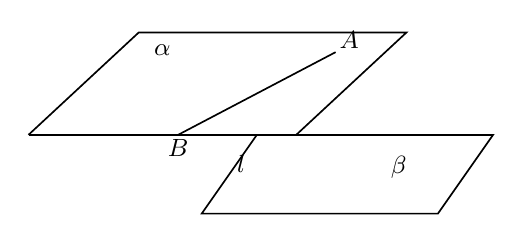
\begin{tikzpicture}[semithick, every node/.style={inner sep=1.2pt, font=\small}]
  % 棱 l
  \draw (-3.00,0) -- (2.90,0);
  % 平面 α（上方）
  \draw (-3.00,0) -- (-1.60,1.30) -- (1.80,1.30) -- (0.40,0);
  % 平面 β（下方）
  \draw (-0.10,0) -- (2.90,0) -- (2.20,-1.00) -- (-0.80,-1.00) -- cycle;
  % AB
  \coordinate (B) at (-1.10,0);
  \coordinate (A) at (0.90,1.05);
  \draw (B) -- (A);
  % 标注
  \node[below] at (-0.30,-0.20) {$l$};
  \node[below] at (B) {$B$};
  \node[above right] at (A) {$A$};
  \node[above] at (-1.30,0.95) {$\alpha$};
  \node[below right] at (1.55,-0.22) {$\beta$};
\end{tikzpicture}
\end{center}
\nopagebreak[4]
\end{question}
\endgroup
\begin{question}
\gkti{16}设 $S$ 为复数集 $\mathbf C$ 的非空子集。若对任意 $x,y\in S$，都有 $x+y$，$x-y$，$xy\in S$，则称 $S$ 为封闭集。下列命题：

① 集合 $S=\{a+b\mathrm i\mid a,b\text{ \text{为整数}},\mathrm i\text{ \text{为虚数单位}}\}$ 为封闭集；

② 若 $S$ 为封闭集，则一定有 $0\in S$；

③ 封闭集一定是无限集；

④ 若 $S$ 为封闭集，则满足 $S\subseteq T\subseteq\mathbf C$ 的任意集合 $T$ 也是封闭集。

其中真命题是$\underline{\qquad}$。（写出所有真命题的序号）

\end{question}
\gkpart{三、解答题}

\begin{question}
\gkti{17}某种有奖销售的饮料，瓶盖内印有“奖励一瓶”或“谢谢购买”字样，购买一瓶若其瓶盖内印有“奖励一瓶”字样即为中奖，中奖概率为 $\dfrac{1}{6}$。甲、乙、丙三位同学每人购买了一瓶该饮料。

（1）求甲中奖且乙、丙都没有中奖的概率；

（2）求中奖人数 $\xi$ 的分布列及数学期望 $E\xi$。

\Needspace{0.4\textheight}
\end{question}
\begingroup
\renewenvironment{question}{\Needspace{0.5\textheight}}{}
\begin{question}
\gkti{18}已知正方体 $ABCD-A'B'C'D'$ 的棱长为 $1$，点 $M$ 是棱 $AA'$ 的中点，点 $O$ 是对角线 $BD'$ 的中点。

（1）求证：$OM$ 为异面直线 $AA'$ 和 $BD'$ 的公垂线；

（2）求二面角 $M-BC'-B'$ 的大小；

（3）求三棱锥 $M-OBC$ 的体积。
\nopagebreak[4]
\begin{center}% 2010 年四川卷理科第 18 题：正方体 ABCD-A'B'C'D'，棱长 1，M 为 AA' 中点，O 为 BD' 中点。
% 来源 PDF：普通高考/2010/2010四川理.pdf，SHA-256 499425696359cfc2cf4418254bdaa1a37487b3dbaa072ff3c7cbe18dbabe73dc。
% 原页：第 1 页（A3 三栏）第 3 栏下部，书页码 631。
% 重绘依据：斜二测投影，竖棱竖直、深度方向斜向上；可见面为前面 ABB'A'、右面 BCC'B'、上面 A'B'C'D'；
%   被遮挡的 AD、DC、DD' 画虚线；MB、BC' 为面内连线（实线），BD'、MO、MC' 为体内连线（虚线）。
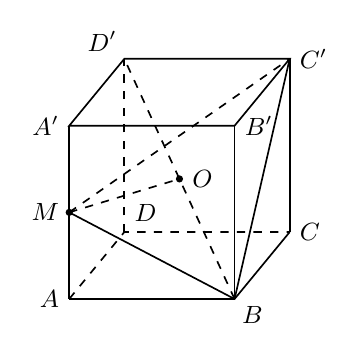
\begin{tikzpicture}[semithick, every node/.style={inner sep=1.4pt, font=\small}]
  \coordinate (A)  at (0.00,0.00);
  \coordinate (B)  at (2.10,0.00);
  \coordinate (C)  at (2.80,0.85);
  \coordinate (D)  at (0.70,0.85);
  \coordinate (A1) at (0.00,2.20);
  \coordinate (B1) at (2.10,2.20);
  \coordinate (C1) at (2.80,3.05);
  \coordinate (D1) at (0.70,3.05);
  \coordinate (M)  at (0.00,1.10);
  \coordinate (O)  at (1.40,1.525);

  % 可见棱
  \draw (A) -- (B) -- (C);
  \draw (C) -- (C1);
  \draw (B) -- (B1);
  \draw (A) -- (A1);
  \draw (A1) -- (B1) -- (C1) -- (D1) -- cycle;

  % 被遮挡的棱
  \draw[dashed] (A) -- (D) -- (C);
  \draw[dashed] (D) -- (D1);

  % 面内连线与体内连线
  \draw (M) -- (B);
  \draw (B) -- (C1);
  \draw[dashed] (B) -- (D1);
  \draw[dashed] (M) -- (O);
  \draw[dashed] (M) -- (C1);

  \fill (M) circle (1.3pt);
  \fill (O) circle (1.3pt);

  % 标注
  \node[left=2pt] at (A) {$A$};
  \node[below right=1pt] at (B) {$B$};
  \node[right=2pt] at (C) {$C$};
  \node[above right=2pt] at (D) {$D$};
  \node[left=2pt] at (A1) {$A'$};
  \node[right=2pt] at (B1) {$B'$};
  \node[right=2pt] at (C1) {$C'$};
  \node[above left=1pt] at (D1) {$D'$};
  \node[left=2pt] at (M) {$M$};
  \node[right=3pt] at (O) {$O$};
\end{tikzpicture}
\end{center}
\nopagebreak[4]
\end{question}
\endgroup
\begin{question}
\gkti{19}（1）① 证明两角和的余弦公式 $C_{(\alpha+\beta)}$：$\cos(\alpha+\beta)=\cos\alpha\cos\beta-\sin\alpha\sin\beta$；

② 由 $C_{(\alpha+\beta)}$ 推导两角和的正弦公式 $S_{(\alpha+\beta)}$：$\sin(\alpha+\beta)=\sin\alpha\cos\beta+\cos\alpha\sin\beta$。

（2）已知 $\triangle ABC$ 的面积 $S=\dfrac{1}{2}$，$\overrightarrow{AB}\cdot\overrightarrow{AC}=3$，且 $\cos B=\dfrac{3}{5}$，求 $\cos C$。

\end{question}
\begin{question}
\gkti{20}已知定点 $A(-1,0)$，$F(2,0)$，定直线 $l:x=\dfrac{1}{2}$，不在 $x$ 轴上的动点 $P$ 与点 $F$ 的距离是它到直线 $l$ 的距离的 $2$ 倍。设点 $P$ 的轨迹为 $E$，过点 $F$ 的直线交 $E$ 于 $B$、$C$ 两点，直线 $AB$、$AC$ 分别交 $l$ 于点 $M$、$N$。

（1）求 $E$ 的方程；

（2）试判断以线段 $MN$ 为直径的圆是否过点 $F$，并说明理由。

\end{question}
\begin{question}
\gkti{21}已知数列 $\{a_n\}$ 满足 $a_1=0$，$a_2=2$，且对任意 $m,n\in\mathbf N^*$ 都有 $a_{2m-1}+a_{2n-1}=2a_{m+n-1}+2(m-n)^2$。

（1）求 $a_3$，$a_5$；

（2）设 $b_n=a_{2n+1}-a_{2n-1}$（$n\in\mathbf N^*$），证明：数列 $\{b_n\}$ 是等差数列；

（3）设 $c_n=(a_{n+1}-a_n)q^{n-1}$（$q\neq0$，$n\in\mathbf N^*$），求数列 $\{c_n\}$ 的前 $n$ 项和 $S_n$。

\end{question}
\begin{question}
\gkti{22}设 $f(x)=\dfrac{1+a^x}{1-a^x}$（$a>0$ 且 $a\neq1$），$g(x)$ 是 $f(x)$ 的反函数。

（1）设关于 $x$ 的方程 $\log_a\dfrac{t}{(x^2-1)(7-x)}=g(x)$ 在区间 $[2,6]$ 上有实数解，求 $t$ 的取值范围；

（2）当 $a=\mathrm e$（$\mathrm e$ 为自然对数的底数）时，证明：$\sum\limits_{k=2}^ng(k)>\dfrac{2-n-n^2}{\sqrt{2n(n+1)}}$；

（3）当 $0<a\leqslant\dfrac{1}{2}$ 时，试比较 $\left|\sum\limits_{k=1}^nf(k)-n\right|$ 与 $4$ 的大小，并说明理由。

\end{question}